\setcounter{chapter}{-1}
% ------------------
\chapter{Unsortiert}
% ------------------

\begin{exercise}
      {ID-3b02cda2482a735aa27ce278c83629ecbcfec0af}
      {Familie}
  \ifproblem\problem
    Vater, Mutter, Tochter und Sohn sind zusammen 73 Jahre alt.
    Der Vater ist drei Jahre älter als die Mutter, die Tochter
    ist 2 Jahre älter als der Sohn. Vor vier Jahren waren
    alle Familienmitglieder zusammen 58 Jahre alt.
    Wie alt sind die Familienmitglieder heute?
  \fi
  %\ifoutline\outline
  %\fi
  %\ifoutcome\outcome
  %\fi
\end{exercise}

\begin{exercise}
      {ID-d7970272ce1b80adf244acbf13201b476eef14b7}
      {Jodlösung}
  \ifproblem\problem
    Eine Lösung von \pc{16} Jod in Alkohol wiegt \sig{735}.
    Es soll eine \pc{10}-ige Jodlösung hergestellt werden.
    Wie viel Gramm Alkohol muss man hinzufügen?
  \fi
  %\ifoutline\outline
  %\fi
  %\ifoutcome\outcome
  %\fi
\end{exercise}

\begin{exercise}
      {ID-c90563e3a7d7f68a59719a773f24e526da443683}
      {Museum}
  \ifproblem\problem
    Die Eintrittskarte in ein Museum kostete \eur{1.50}. Nachdem der Eintrittspreis
    gesenkt wurde, wuchsen die Besucherzahlen um \pc{50} und die Einnahmen um \pc{25}.
    Um wie viel Cent pro Karte wurde der Preis verringert?
  \fi
  %\ifoutline\outline
  %\fi
  %\ifoutcome\outcome
  %\fi
\end{exercise}

\begin{exercise}
      {ID-812972e6c6b1b8e11b6ad6d09d94a0a8430c6d93}
      {Summe}
  \ifproblem\problem
    In einer Summe ist der erste Summand $\frac{5}{12}$ des zweiten Summanden.
    Wie viel Prozent der Summe entfällt auf den kleineren Summanden?
  \fi
  %\ifoutline\outline
  %\fi
  %\ifoutcome\outcome
  %\fi
\end{exercise}

\begin{exercise}
      {ID-50c3c2e404df3294991c0c6e283d7445e34ee7e1}
      {Das Floß}
  \ifproblem\problem
    Ein Motorboot, das auf einem Fluss zwischen den Städten $A$ und $B$ pendelt,
    benötigt für die Fahrt flussabwärts 32 Stunden. Die Rückfahrt von $B$ nach
    $A$ dauert 48 Stunden. In wie vielen Stunden bewegt sich ein Floß von $A$
    nach $B$?
  \fi
  %\ifoutline\outline
  %\fi
  %\ifoutcome\outcome
  %\fi
\end{exercise}

\begin{exercise}
      {ID-f6c038f6558edd5ad9fb7e0aa8052eb9f5650393}
      {Die Flasche}
  \ifproblem\problem
    Ein Sportler schwimmt gegen den Strom in einem Fluss und verliert unter
    einer Brücke eine Flasche. Ohne den Verlust zu bemerken schwimmt er
    zunächst noch eine viertel Stunde weiter. Als er bemerkt, dass er seine
    Flasche verloren hat, schwimmt er zurück und holt sie \sikm{2} von der
    Brücke entfernt wieder ein. Ermittle die Strömungsgeschwindigkeit des
    Flusses.
  \fi
  %\ifoutline\outline
  %\fi
  %\ifoutcome\outcome
  %\fi
\end{exercise}

\begin{exercise}
      {ID-b3894022b7915d3462db4b9497701ab0ec2f5750}
      {Zügig}
  \ifproblem\problem
    Ein Zug fährt im Bahnhof innerhalb von $t_{1}$ Sekunden an einer Person vorbei.
    Danach fährt derselbe Zug innerhalb von $t_{2}$ Sekunden über eine benachbarte,
    $a$ Meter lange Brücke. Die Zeit zum Überqueren der Brücke wird von dem Zeitpunkt
    an gemessen, an dem die Spitze des Zuges die Brücke erreicht, bis zu dem
    Zeitpunkt, an dem das Ende des Zuges die Brücke verlässt.
    Ermittle die Länge und die Geschwindigkeit des Zuges in Anbhängigkeit von $t_{1}$,
    $t_{2}$ und $a$.
  \fi
  %\ifoutline\outline
  %\fi
  %\ifoutcome\outcome
  %\fi
\end{exercise}

\begin{exercise}
      {ID-0a39950ace00a7c5ec3c0db4d6873aae39deb51a}
      {Der Weg in die Stadt}
  \ifproblem\problem
    Ein Dorf liegt \sikm{48} von der nächsten Stadt entfernt. Im Dorf starten zeitgleich
    ein Bauer auf einem Pferd und ein Briefträger auf einem Fahrrad ihren Weg in die Stadt.
    Das Pferd läuft mit einer Durchschnittsgeschwindigkeit von \sikmh{7}, der Briefträger
    schafft auf seinem Fahrrad duchschnittlich \sikmh{13}. Nach wie vielen Stunden beträgt
    der verbleibende Weg bis zur Stadt für den Briefträger nur noch ein Drittel des für
    den Bauern verbleibenden Weges?
  \fi
  %\ifoutline\outline
  %\fi
  %\ifoutcome\outcome
  %\fi
\end{exercise}

\begin{exercise}
      {ID-fffc17cb928a23befe424d29a4c070d9d80648be}
      {Schulweg}
  \ifproblem\problem
    Zwei Kinder, die im selben Haus wohnen, gehen gemeinsam in die gleiche
    Schule. Das erste Kind geht die Hälfte der Zeit mit einer
    Durchschnittsgeschwindigkeit von \sikmh{5}, danach mit \sikm{4}. Das
    zweite Kind geht die Hälfte des Weges mit einer Durchschnittsgeschwindigkeit
    von \sikmh{4}, danach mit \sikmh{5}. Welches Kind erreicht die Schule
    zuerst?
  \fi
  %\ifoutline\outline
  %\fi
  %\ifoutcome\outcome
  %\fi
\end{exercise}

\begin{exercise}
      {ID-e9db77c9a5bbbfd8e37ea60ee54738c90e3cccfc}
      {Schrittlänge}
  \ifproblem\problem
    Vater und Sohn messen mit ihren Schritten den Abstand zwischen zwei Bäumen.
    Zuerst schreitet der Vater die Strecke ab, danach sein Sohn. Als der Sohn
    losgeht, ist auf dem Boden die Spur des Vaters deutlich zu erkennen.
    Der Sohn tritt insgesamt 10 Mal genau auf den Fußabdruck seines Vaters --
    zum Glück auch am Ende der Strecke. Ein Schritt des Vaters ist \sicm{70}
    lang, ein Schritt des Sohnes misst \sicm{56}. Wie weit sind die beiden
    Bäume voneinander entfernt?
  \fi
  \ifoutline\outline
    Vielleicht hilft das kleinste gemeinsame Vielfache\ldots
  \fi
  %\ifoutcome\outcome
  %\fi
\end{exercise}

\begin{exercise}
      {ID-11355ef27a46bdeef9e283bbbd480a94e14eb326}
      {Parallelogramm}
  \ifproblem\problem
    Gegeben sei ein beliebiges (konvexes) Viereck. Zerschneide es so in vier
    kleinere Vierecke, dass man daraus ein (gleich großes) Parallelogramm legen
    kann.
  \fi
  %\ifoutline\outline
  %\fi
  %\ifoutcome\outcome
  %\fi
\end{exercise}

\begin{exercise}
      {ID-c5b39ea16827187dcc3c7a2fdcc009495a327bff}
      {Drei Buslinien}
  \ifproblem\problem
    Um 6 Uhr morgens starten drei Busse gleichzeitig vom Bahnhof einer Stadt.
    Sie fahren bis spätestens 22 Uhr abends.\par
    Für eine Runde benötigt
    der erste Bus eine Stunde und 30 Minuten,
    der zweite Bus eine Stunde und 50 Minuten und
    der dritte Bus eine Stunde und 10 Minuten.
    Nach jeder Runde machen sie 10 Minuten Pause.
    Wann starten
    \begin{enumerate}[a)]
      \item der erste und der zweite Bus
      \item der zweite und der dritte Bus
      \item alle drei Busse
    \end{enumerate}
    wieder gleichzeitig vom Bahnhof?
  \fi
  %\ifoutline\outline
  %\fi
  %\ifoutcome\outcome
  %\fi
\end{exercise}

\begin{exercise}
      {ID-bd8671ab6df925a373f03c9f55ebf12674dbc594}
      {Freundschaft}
  \ifproblem\problem
    In einer Klasse sind 27 Schüler. Jeder Junge ist mit 4 Mädchen befreundet
    und jedes Mädchen ist mit 5 Jungen befreundet. Wie viele Mädchen und wie
    viele Jungen sind in der Klasse?
  \fi
  %\ifoutline\outline
  %\fi
  %\ifoutcome\outcome
  %\fi
\end{exercise}

\begin{exercise}
      {ID-cd6ac26505aaa68d1570175c5645e808e33ac82f}
      {Unendlich viele Dreiecke}
  \newcommand{\topdowntriangle}[3]
  {%
    % zeichne ein graues, auf dem Kopf stehendes, gleichseitiges Dreieck
    \filldraw[fill=black!40!white] (#1, #2) -- ++(60:#3) -- ++(180:#3) -- cycle;
  }%
  \ifproblem\problem
    Die folgende Abbildung zeigt gleichseitige Dreiecke. Das größte (äußere) Dreieck
    besitzt den Flächeninhalt 1.
    \begin{center}
      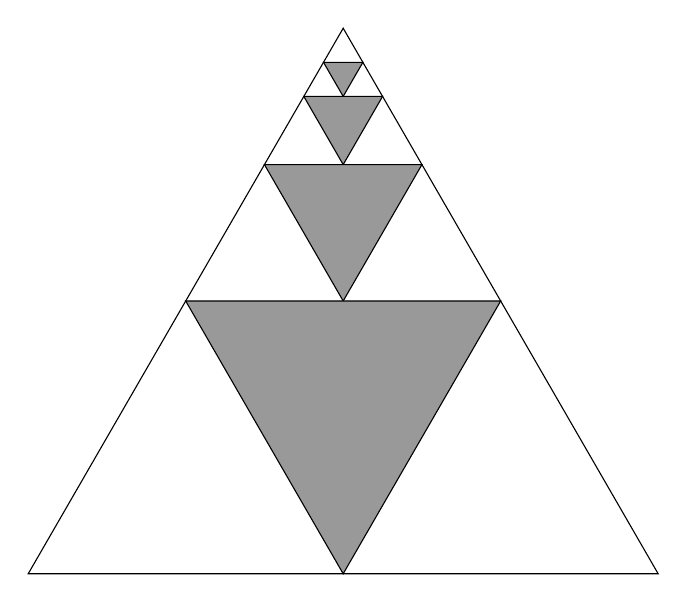
\begin{tikzpicture}[scale=0.5]
        \topdowntriangle{0}{12.12435}{1};
        \topdowntriangle{0}{10.3923}{2};
        \topdowntriangle{0}{6.9282}{4};
        \topdowntriangle{0}{0}{8};
        \draw (-8, 0) -- (8, 0) -- ++(120:16) -- cycle;
      \end{tikzpicture}
    \end{center}
    \begin{enumerate}[a)]
      \item Berechne den gemeinsamen Flächeninhalt der 4 grauen Dreiecke.
      \item Angenommen, man setzt die Konstruktion der grauen Dreiecke
            unendlich oft nach oben in die Spitze des äußeren Dreiecks fort.
            Wie groß wird dann die gemeinsame graue Fläche letztendlich werden?
    \end{enumerate}
  \fi
  \ifoutline\outline
    Vielleicht hilft es, wenn man in \textit{Trapezen} denkt statt in \textit{Dreiecken}\ldots
  \fi
  \ifoutcome\outcome
    Letztendlich beträgt der Flächeninhat der grau gefärbten Fläche $\frac{1}{3}$.
    Drei benachbarte Dreiecke bilden in jeder \glqq Reihe\grqq{} ein Trapez.
    Von jedem dieser Trapeze ist ein Drittel grau gefärbt, also ist letztendlich
    auch ein Drittel des großen Dreiecks grau gefärbt.
  \fi
\end{exercise}

% stop here...
%\end{document}

